\chapter{静态无向模型}
\label{chap:pgm-energy-models}

第~\ref{chap:pgm-static-directed}章的模型都建立在有向图上：每个变量都有一组明确的“父变量”，联合分布被写成一串条件概率的乘积，这天然对应“谁生成谁”的过程。但在很多问题里，变量之间只有\emph{相互相容、彼此约束}的对称关系，很难说谁是因谁是果：一排相邻测温点倾向于同时过热或同时正常，图像里相邻像素倾向于颜色相近，一条流水线上的标签倾向于彼此一致。给这种关系硬安一个箭头方向会很随意，而且不同方向可能表达的是同一个分布。无向模型正是为这类“状态之间的相容性”准备的：它不为变量指定生成方向，而是直接对\emph{整组状态配置}打分——越符合局部相容偏好的配置权重越高，再用一个全局归一化常数把所有配置的权重折算成概率。

这套“先打分、再全局归一化”的做法带来一个贯穿全章的特点，也是它和有向模型最实际的差别：有向模型的每个局部条件分布各自归一化，学参数时常常数一数计数即可；无向模型的局部势\emph{不}各自归一化，所有配置共享一个配分函数，于是无论做推断还是学习，都绕不开一次对全部配置的求和（或积分）。本章的一个核心关注点，就是这个配分函数在不同结构下何时可算、何时必须借助采样或近似，以及哪些建模选择能避开它。

相邻检测位置可能同时过热，也可能受到同一测量干扰，整排状态因而需要联合考虑。给定各位置的相对偏好以及相邻状态的相容权重，怎样计算整排配置的概率？若温度读数已知、只需预测异常标签，是否还要同时建立这些读数的生成分布？对第二个问题的不同回答把本章分成两大块：如果要为全部变量建立联合分布，就对所有状态配置归一化（联合无向模型，如Ising、玻尔兹曼机）；如果输入已知、只预测一组相互关联的标签，就把输入固定、只在标签空间归一化（条件无向模型，如条件随机场），从而免去为输入本身建模的负担。联合无向模型比较全部建模变量的配置，条件无向模型则固定输入、只比较输出。局部无向分解规定了变量在给定分隔节点后的独立关系（参见第~\ref{chap:pgm-undirected}章）；本章据此构造具体模型，说明结构怎样影响推断，以及潜变量、高阶势和神经参数化各带来哪些表达能力与计算要求。联合与条件是本章的主要划分；变量是否可见、势是否成对以及参数化方式可以组合。

\section{局部相容关系的概率建模问题}
\label{sec:pgm-energy-models-common}

本节建立无向模型的三个共同对象：用局部势给团上的状态打分、把这些分数写成能量形式的概率，以及用全局配分函数归一化。后续Ising、高斯和玻尔兹曼机分别为能量选择不同的具体函数形式。设无向图为$\mathcal{G}=(V,E)$，令$d=|V|$、$\bm{X}=(X_1,\ldots,X_d)^\top$。团是一小群相互关联的变量；团上的每种局部状态配置对应一个非负相对权重，配置越符合建模偏好（相邻状态越相容），权重越大。权重不要求自身求和为$1$。配置越符合建模偏好，其\term{势函数}（potential function）值越大。记因子作用域集合为$\mathcal{C}$，每个$C\in\mathcal{C}$取图中的一个团，允许使用非极大团。将严格正势$\psi_{\bm{\theta},C}$写成局部能量$E_{\bm{\theta},C}=-\log\psi_{\bm{\theta},C}$，乘积权重便转为能量之和：
\begin{equation}
  \begin{aligned}
    E_{\bm{\theta}}(\bm{x})
      &=\sum_{C\in\mathcal{C}}E_{\bm{\theta},C}(\bm{x}_C),\\
    p_{\bm{\theta}}(\bm{x})
      &=\frac{\prod_{C\in\mathcal{C}}
               \psi_{\bm{\theta},C}(\bm{x}_C)}
              {Z_{\bm{\theta}}}
        =\frac{\exp[-E_{\bm{\theta}}(\bm{x})]}{Z_{\bm{\theta}}},\\
    Z_{\bm{\theta}}
      &=\int \exp[-E_{\bm{\theta}}(\bm{u})]\,\mathrm{d}\mu(\bm{u}).
  \end{aligned}
  \label{eq:pgm-energy-models-joint}
\end{equation}
参数向量$\bm{\theta}$包含各局部势的参数。离散状态采用计数测度$\mu$，连续状态采用指定基准测度，通常是Lebesgue测度。之所以把势取负对数、改写成“能量”，一是因为对数能把各团势的\emph{乘积}变成能量的\emph{求和}，便于优化和求导；二是这个写法直接借自统计物理：物理系统倾向于处在能量低的状态，这里则让“越相容”的配置能量越低、概率越大，玻尔兹曼分布$e^{-E}$正是这个意思，“玻尔兹曼机”等名称也由此而来。但$e^{-E}$本身一般不构成概率，因为它对所有配置求和不等于$1$；必须除以这个总和才能归一化。\term{能量函数}（energy function）的值越低，配置的未归一化权重越大；\term{配分函数}（partition function）$Z_{\bm{\theta}}$累加或积分全部权重，使其成为概率，故须满足$0<Z_{\bm{\theta}}<\infty$。这里使用无量纲的对数权重，物理模型的逆温度已计入参数。

也可以用负能量$f_{\bm{\theta}}=-E_{\bm{\theta}}$给配置评分，对数概率还需扣除$\log Z_{\bm{\theta}}$。增加与$\bm{x}$无关的能量常数，会等比例缩放全部权重及配分函数，概率保持原值。按正比例缩放能量时，配置间的能量差也同比例变化；比例不为$1$且两个配置的能量不同时，它们的概率比会改变。若只比较固定模型中的两种配置，配分函数可从比值中消去：
\[
  \frac{p_{\bm{\theta}}(\bm{x})}{p_{\bm{\theta}}(\bm{x}')}
  =\exp\{E_{\bm{\theta}}(\bm{x}')-E_{\bm{\theta}}(\bm{x})\}.
\]
因此，能量差能够排序配置，绝对概率仍依赖全部权重的总量。改变局部势的状态偏好时，配分函数也可能改变；即使某个配置的未归一化权重不变，其概率仍可能随归一化而改变。

若测量输入$\bm{x}$已经固定、待预测量为$\bm{Y}$，需要比较的候选只有输出配置。相同能量构造此时只在输出空间归一化：
\begin{equation}
  \begin{aligned}
    p_{\bm{\theta}}(\bm{y}\mid\bm{x})
      &=\frac{\exp[-E_{\bm{\theta}}(\bm{y},\bm{x})]}
              {Z_{\bm{\theta}}(\bm{x})},\\
    Z_{\bm{\theta}}(\bm{x})
      &=\int\exp[-E_{\bm{\theta}}(\bm{v},\bm{x})]
                  \,\mathrm{d}\mu_Y(\bm{v}).
  \end{aligned}
  \label{eq:pgm-energy-models-conditional}
\end{equation}
每个使用的输入都须给出$0<Z_{\bm{\theta}}(\bm{x})<\infty$。该式只定义输出的条件概率，没有为输入规定$p(\bm{x})$，也不限制输入之间的依赖。附加只依赖输入的能量$c(\bm{x})$时，它在分子、分母中消去。图~\ref{fig:pgm-energy-models-normalization}据此区分输入的两种职责：它可以改变各势的数值，却不参与输出的求和。

\begin{figure}[htbp]
  \centering
  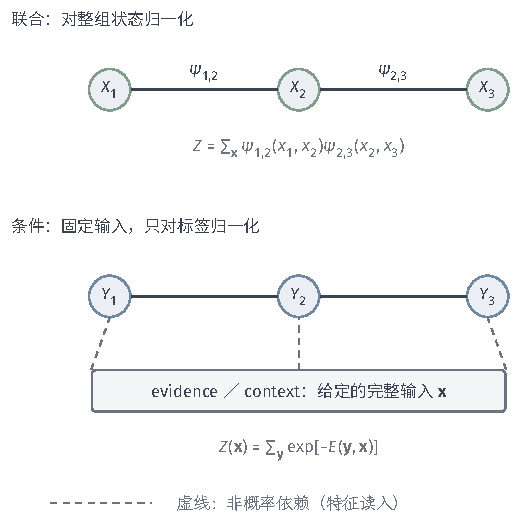
\includegraphics[width=86.907mm]{figures/09-probabilistic-graphical-models/04-models/tikz/pgm-energy-models-normalization/figure.pdf}
  \caption{三节点相互作用的两种归一化。上方联合模型对全部状态求和；下方把$\bm{x}$列为给定证据或条件输入，只对标签$\bm{y}$求和。灰底框中的输入通过虚线影响标签势，虚线表示特征依赖，不表示有向生成关系。}
  \label{fig:pgm-energy-models-normalization}
\end{figure}

有限离散状态配合有限能量，必然产生正且有限的配分函数。连续能量则需检查尾部：即使$E(x)=-x^2$处处有定义，$\int_{\mathbb{R}}e^{x^2}\,\mathrm{d}x$仍发散。允许势为零时，可以用$+\infty$能量排除配置，但归一化还须有正总权重；离散支持至少保留一个正权配置，连续支持则需有正测度。因子分解仍能给出相应Markov性质，而从Markov性质反推分解的正性定理不能直接用于零势（参见第~\ref{chap:pgm-undirected}章）。

若要从观测数据确定能量参数，还需要规定学习目标，而不仅是为配置打分。设完整观测记录为$\{\bm{x}_r\}_{r=1}^n$，并把这些记录视为来自同一分布的独立样本；每条记录内部的节点仍可相关。最大似然等价于最小化负对数似然
\begin{equation}
  \mathcal{L}(\bm{\theta})
    =\sum_{r=1}^nE_{\bm{\theta}}(\bm{x}_r)
       +n\log Z_{\bm{\theta}}.
  \label{eq:pgm-energy-models-common-nll}
\end{equation}
第一项鼓励降低数据配置的能量，第二项约束全部配置的总权重，防止模型只靠整体降低能量来改善目标。在能交换微分与积分、相关期望有限的条件下，其梯度为
\[
  \nabla_{\bm{\theta}}\mathcal{L}
   =\sum_{r=1}^n\nabla_{\bm{\theta}}E_{\bm{\theta}}(\bm{x}_r)
    -n\mathbb{E}_{p_{\bm{\theta}}}
          [\nabla_{\bm{\theta}}E_{\bm{\theta}}(\bm{X})].
\]
模型期望来自配分函数的导数；忽略它会改变学习目标。若部分状态未观测，梯度中的第一项也要对给定数据的隐藏后验求期望。条件模型则把每条记录的$\log Z_{\bm{\theta}}$换成$\log Z_{\bm{\theta}}(\bm{x}_r)$，模型期望相应只在该输入的输出空间计算。下面将分别写出各模型中的统计量和更新办法，通用梯度推导可参见第~\ref{chap:pgm-parameter-learning}章。

\section{联合状态分布的构造与学习}
\label{sec:pgm-energy-models-joint-models}

为整组测量状态建立联合分布，可以用于补全状态、计算多变量事件概率或生成配置。构造这类分布有两条路径：一条直接为待建模状态指定能量，另一条先让可见状态与隐藏状态共同参与能量，再把隐藏状态求和消去。两条路径都使用式~\eqref{eq:pgm-energy-models-joint}，区别在于需要在哪些变量上计算权重、后验和配分函数。

\subsection{直接对状态配置赋能量}
\label{sec:pgm-energy-models-pairwise}

有了能量这个通用语言，最自然的第一个具体模型出现在每个变量只有两种状态时（正常/异常、开/关、像素黑/白）。它最早由物理学家Ising用来描述磁铁中相邻原子的自旋是否同向，后来成为二值无向模型的标准原型：能量只由两类最简单的项组成——每个位置自身更偏向哪个状态（一元项），以及每对相邻位置更希望同向还是反向（成对项）。下面先从二值和多类别的成对作用出发，再考察连续二次能量、整组约束、神经参数化和逻辑模板。后几项改变的是不同方面，因而可以组合：高阶势可以由神经网络计算，也可以按照关系模板在多个实体组之间共享参数。

\subsubsection{Ising：用一元偏好和同异号作用描述二值状态}
\label{sec:pgm-energy-models-ising}

把两种状态记为$x_i\in\{-1,+1\}$（像自旋朝上/朝下）有一个特别的便利：两个状态“是否同向”恰好可以用乘积$x_ix_j$表示——同向时为$+1$、异号时为$-1$，于是“奖励同向或异号”就能用一个参数乘上这个乘积线性地写出来。对只有两种状态的检测位置，\term{Ising模型}（Ising model）分别用单点参数表示状态偏好，用边参数表示相邻状态同号或异号的偏好：
\begin{equation}
  E_{\bm{\theta}}(\bm{x})
    =-\sum_{i\in V}b_ix_i
     -\sum_{\{i,j\}\in E}J_{i,j}x_ix_j.
  \label{eq:pgm-energy-models-ising}
\end{equation}
\term{外场}（external field）$b_i$取正值时偏好$+1$。\term{耦合参数}（coupling parameter）$J_{i,j}$取正值时奖励同号，取负值时奖励异号；每条无向边只计一次，约定$J_{i,j}=J_{j,i}$。这些参数描述统计相容性，不能仅凭它们推断干预一个位置对另一位置的效应。

要计算一个位置的条件概率，固定其余状态，仅保留含$x_i$的得分$x_i(b_i+\sum_{j\in N(i)}J_{i,j}x_j)$，其中$N(i)$为邻居集合。$+1$与$-1$的权重比为$\exp[2(b_i+\sum_jJ_{i,j}x_j)]$，归一化两项后得到
\begin{equation}
  \begin{aligned}
    p_{\bm{\theta}}(X_i=+1\mid\bm{x}_{V\setminus\{i\}})
      &=\sigma\!\left(2b_i+
           2\sum_{j\in N(i)}J_{i,j}x_j\right),\\
    \sigma(u)&=\frac{1}{1+e^{-u}}.
  \end{aligned}
  \label{eq:pgm-energy-models-ising-conditional}
\end{equation}
这个满条件分布只读取邻居状态。移去这些条件以后，无直接边的两个节点仍可能经其他节点相关。

用三个相邻位置构造数值例子：图取$1-2-3$，不设单点偏好，同号边势为$3$、异号边势为$1$。这些是人为指定的权重，尚未归一化为概率。为计算联合权重，先统计相邻同号对：
\[
  N_{=}(\bm{x})
   =\mathbf{1}\{x_1=x_2\}+\mathbf{1}\{x_2=x_3\}.
\]
令$E_0(\bm{x})=-(\log3)N_{=}(\bm{x})$，配置权重就是$3^{N_{=}(\bm{x})}$。首节点可取两个值，每个后继节点的两项权重和为$3+1=4$，故$Z_0=2\times4\times4=32$。由$\mathbf{1}\{x_i=x_j\}=(1+x_ix_j)/2$，这也对应$J_{1,2}=J_{2,3}=(\log3)/2$的Ising分布。两种能量约定相差常数：$E_0$比式~\eqref{eq:pgm-energy-models-ising}的零外场能量少$\log3$，后者的配分函数为$32/3$。概率相同，配分函数数值则随能量常数而变。

在该对称链中，给定一个位置，后继位置同号和异号的条件概率分别为$3/4$、$1/4$。两端同号对应两次保持或两次翻转，因而
\[
  p(X_3=X_1\mid X_1)
    =(3/4)^2+(1/4)^2=\frac58.
\]
各节点的边缘都为均匀二值分布，所以$\mathbb{E}[X_1X_3]=2(5/8)-1=1/4$。两端虽无边仍相关，给定$X_2$才独立。将同样参数用于更长的零外场链，每跨一条边，条件均值乘以$1/2$，相隔$r$条边的相关为$(1/2)^r$。这说明相互作用能够沿路径传递，其强度还由参数决定。

这些参数可以由完整观测配置学习。把第$r$条记录的节点状态记为$x_{r,i}$，固定图上的Ising对数似然为
\begin{equation}
  \begin{aligned}
  \ell_{\mathrm{I}}(\bm{b},\bm{J})
   &=\sum_{r=1}^n\left[
        \sum_i b_i x_{r,i}
        +\sum_{\{i,j\}\in E}J_{i,j}x_{r,i}x_{r,j}\right]\\
   &\quad-n\log Z_{\bm{b},\bm{J}}.
  \end{aligned}
  \label{eq:pgm-energy-models-ising-likelihood}
\end{equation}
节点偏好与边相容性分别对应一阶、二阶统计，梯度因而为
\[
  \begin{aligned}
    \frac{\partial\ell_{\mathrm{I}}}{\partial b_i}
      &=\sum_{r=1}^n x_{r,i}-n\mathbb{E}[X_i],\\
    \frac{\partial\ell_{\mathrm{I}}}{\partial J_{i,j}}
      &=\sum_{r=1}^n x_{r,i}x_{r,j}-n\mathbb{E}[X_iX_j].
  \end{aligned}
\]
这里的期望均在当前参数的联合模型下取得。一次学习迭代先固定参数计算节点边缘和边上的联合边缘统计，再选择合适步长沿上述梯度方向更新；例如以步长$\eta>0$更新$J_{i,j}\leftarrow J_{i,j}+\eta\,\partial\ell_{\mathrm{I}}/\partial J_{i,j}$。小图可以枚举，树可以传递消息，一般图则可能需要近似推断或采样。固定图且存在有限内点最大似然解时，零梯度意味着相应模型期望与经验统计量匹配。

式~\eqref{eq:pgm-energy-models-ising-conditional}还给出一种无需联合配分函数的拟合办法：最大化伪对数似然
\[
  \ell_{\mathrm{PL}}(\bm{b},\bm{J})
    =\sum_{r=1}^n\sum_{i\in V}
       \log p_{\bm{b},\bm{J}}
           (x_{r,i}\mid\bm{x}_{r,V\setminus\{i\}}).
\]
每个条件概率只归一化两个状态，可以直接求导并更新共享的节点、边参数。这个目标比较观测节点与其已知邻居下的两个候选状态，并不等于联合似然；把节点条件项相乘也不使同一记录中的节点变成独立样本。能否准确恢复真实参数，还取决于模型是否能表达真实分布、样本获取方式及样本量，不能仅由满条件可算推出。相同满条件也可用于Gibbs采样，但强耦合时单点变化难以转到另一种整体配置，解析更新并不保证快速混合。

\subsubsection{Potts：让类别相容性不依赖标签数字}
\label{sec:pgm-energy-models-potts}

当状态不止两种（比如一个位置属于$K$个故障类别之一）时，$x_ix_j$这种“标签编号相乘”的写法就失效了：类别编号只是名字，把“类别1”和“类别3”相乘毫无意义，编号怎么排也不应影响模型。正确的做法是不看编号数字，只看两个位置的类别\emph{是否相同}，用一个示性函数来奖励“同类相邻”。类别数增加到$K>2$后，标签编号的乘积无法直接表示相容性。\term{Potts模型}（Potts model）改为比较类别是否相等，对$x_i\in\{1,\ldots,K\}$定义
\begin{equation}
  E_{\bm{\theta}}(\bm{x})
   =-\sum_i b_i(x_i)
    -\sum_{\{i,j\}\in E}J_{i,j}\mathbf{1}\{x_i=x_j\}.
  \label{eq:pgm-energy-models-potts}
\end{equation}
$b_i(k)$规定位置$i$对类别$k$的偏好。计算节点条件分布时，固定邻居，为每个类别$k$形成权重
\[
  w_i(k)=\exp\left\{
    b_i(k)+\sum_{j\in N(i)}J_{i,j}\mathbf{1}\{k=x_j\}
  \right\},
\]
将权重除以$\sum_{\ell=1}^K w_i(\ell)$即得满条件概率。每条边只用一个参数区分类别相同与不同，限制了它能表达的相容关系；特定异类组合有不同偏好时，需改用$K\times K$边势表。二类Potts可以重新编码为Ising：将两类改记为$\widetilde{x}_i\in\{-1,+1\}$，则$\mathbf{1}\{x_i=x_j\}=(1+\widetilde{x}_i\widetilde{x}_j)/2$，Ising耦合为Potts耦合的一半。相应外场为两类一元得分之差的一半，其余项并入能量常数。这里既改变编码，也换算参数，不能只更换模型名称。

给定完整类别配置，Potts模型最大化
\begin{equation}
  \begin{aligned}
  \ell_{\mathrm{P}}(\bm{b},\bm{J})
   &=\sum_{r=1}^n\left[
       \sum_i b_i(x_{r,i})+
       \sum_{\{i,j\}\in E}J_{i,j}
               \mathbf{1}\{x_{r,i}=x_{r,j}\}\right]\\
   &\quad-n\log Z_{\bm{b},\bm{J}}.
  \end{aligned}
  \label{eq:pgm-energy-models-potts-likelihood}
\end{equation}
两类参数需要的统计量变为类别指示与同类指示：
\[
  \begin{aligned}
    \frac{\partial\ell_{\mathrm{P}}}{\partial b_i(k)}
      &=\sum_r\mathbf{1}\{x_{r,i}=k\}
          -n\,p_{\bm{b},\bm{J}}(X_i=k),\\
    \frac{\partial\ell_{\mathrm{P}}}{\partial J_{i,j}}
      &=\sum_r\mathbf{1}\{x_{r,i}=x_{r,j}\}
          -n\,p_{\bm{b},\bm{J}}(X_i=X_j).
  \end{aligned}
\]
学习时先计算当前模型的节点与边缘概率，再用观测统计减模型统计做梯度上升。每个位置的一元得分同时加常数不改变分布，可固定一个参考类别得分以消除这项冗余。训练后，归一化的$w_i(k)$可用于局部补全或Gibbs更新；联合事件概率仍需全局推断。若使用一般$K\times K$边势，各类别对都要有相应统计量，已经超出这里用单一参数奖励同类的Potts形式。

一般稠密边势在树上求配分函数与边缘需$O(dK^2)$运算，特殊边势可能进一步简化。一般图则受消元后的诱导宽度限制，原始因子成对不保证全局计算只有二次成本。二值吸引型模型可以通过图割求最优配置，但这一最大化未计算配分函数（参见第~\ref{chap:pgm-variational}章）。参数也会限制模型适用性：过强的同号偏好可能掩盖局部异常；三角形的每条边都偏好异号时，任一二值配置至少违背一项偏好。

\subsubsection{GMRF：用二次能量表达连续条件依赖}
\label{sec:pgm-energy-models-gmrf}

对连续状态，最自然的能量形式是关于状态的二次函数（就像弹簧的势能）：偏离均值越远能量越高，交叉项刻画两个位置共同变化的相容程度。二次能量的巨大好处是配分函数恰好是一个高斯积分、可以\emph{解析}算出，不必像离散模型那样枚举全部配置——这同时说明为什么连续无向模型几乎都与高斯分布绑定。温度读数是连续量，二值或类别相同与否已不足以刻画其变化幅度。可以用二次能量惩罚状态偏离均值，并用交叉项描述多个位置共同变化的相容程度；这样既保留相互作用，又能够通过高斯积分取得归一化概率。\term{高斯Markov随机场}（Gaussian Markov random field, GMRF）通过精度矩阵表示条件依赖；对$\bm{x}\in\mathbb{R}^d$取
\begin{equation}
  \begin{aligned}
    E_{\bm{\theta}}(\bm{x})
      &=\frac12(\bm{x}-\bm{\mu})^\top
                    \bm{Q}(\bm{x}-\bm{\mu}),\\
    Z_{\bm{\theta}}
      &=(2\pi)^{d/2}|\bm{Q}|^{-1/2},
      \qquad \bm{Q}=\bm{Q}^\top\succ0.
  \end{aligned}
  \label{eq:pgm-energy-models-gaussian}
\end{equation}
均值为$\bm{\mu}$，协方差的逆$\bm{Q}$称为\term{精度矩阵}（precision matrix）。正定性使二次能量在所有方向增长，并使高斯积分有限。为补全一个未知位置，给定其余位置后的分布为
\[
  \begin{aligned}
    \widetilde{\mu}_i(\bm{x})
      &=\mu_i-\frac{1}{Q_{i,i}}
           \sum_{j\ne i}Q_{i,j}(x_j-\mu_j),\\
    X_i\mid\bm{x}_{V\setminus\{i\}}
      &\sim\mathcal{N}\!\left(
          \widetilde{\mu}_i(\bm{x}),Q_{i,i}^{-1}\right).
  \end{aligned}
\]
$\widetilde{\mu}_i$是给定其余节点后的条件均值。在非退化高斯模型中，对不同节点$i,j$，$Q_{i,j}=0$恰好对应$X_i\perp X_j\mid\bm{X}_{V\setminus\{i,j\}}$；协方差为零判别的则是边缘独立，两者不可互换（证明参见第~\ref{chap:pgm-undirected}章）。

仍取三个检测位置，用中心化并缩放后的温度构造零均值模型，令
\[
  \bm{Q}=
  \begin{pmatrix}
    2&-1&0\\ -1&2&-1\\ 0&-1&2
  \end{pmatrix},
  \qquad
  \bm{Q}^{-1}=\frac14
  \begin{pmatrix}
    3&2&1\\ 2&4&2\\ 1&2&3
  \end{pmatrix}.
\]
$\bm{Q}$的顺序主子式为$2,3,4$，所以它正定。两端精度为零，协方差却为$1/4$，展示了中点传递的边缘相关。给定$x_1=2,x_3=0$，中点分布为$\mathcal{N}(1,1/2)$；以条件均值补全得到$1$，条件方差则量化补全后仍有的不确定性。

高斯推断主要使用线性求解和矩阵分解。稠密Cholesky分解耗时$O(d^3)$，随后可计算条件均值、所需协方差及对数行列式；链状精度具有固定带宽时，分解可随$d$线性增长。一般稀疏矩阵可能产生消元填充，原始零元素数量因此不足以判定时间成本。学习时，若均值已知为零，取样本二阶矩$\bm{S}=n^{-1}\sum_{r=1}^n\bm{x}_r\bm{x}_r^\top$，要最大化的精度相关对数似然为
\[
  \frac n2\{\log|\bm{Q}|-\operatorname{tr}(\bm{S}\bm{Q})\},
  \qquad \bm{Q}\succ0,
\]
缺边对应$Q_{i,j}=0$，这些约束与正定性共同限定候选精度。均值已知为一般$\bm{\mu}$时，$\bm{S}$改用以该均值中心化的二阶矩；均值也待估且样本完整时，可以先取样本均值，再用相应的中心化样本协方差求精度。矩阵梯度为$\frac n2(\bm{Q}^{-1}-\bm{S})$。无图约束且$\bm{S}\succ0$时，令梯度为零即得最优解$\bm{S}^{-1}$。

有零约束时，通常在允许的对角与边坐标上优化：先以当前正定$\bm{Q}$求解所需的$\bm{Q}^{-1}$元素，再由模型协方差减经验协方差构造上升方向，并选择保持正定、提高目标值的步长。直接把$\bm{S}^{-1}$的禁用元素置零不等价于这个约束问题，也不能保证所得矩阵正定。训练后的精度用于条件补全，或通过高斯分解生成整组状态；这两种用途依赖同一个已经归一化的高斯分布。

仅半正定的精度不能在整个$\mathbb{R}^d$上归一化为式~\eqref{eq:pgm-energy-models-gaussian}，单个高斯也无法表达多峰。解析计算的便利伴随这些表示条件，延长优化迭代不能消除它们\scite{pgm-undirected-rue2005}

这里约束的是精度矩阵中的零，前章因子分析与概率PCA约束的则是协方差的低秩加对角形式。前者用条件独立性描述哪些位置需要直接相互作用，后者用少量隐藏因子解释共同变化；稀疏精度的逆通常并不稀疏，低秩加对角协方差的逆也未必满足给定缺边。固定稀疏图和低维潜变量维数后，这两种受限模型族一般不互相包含；若允许完整精度图，则任何非退化因子分析或概率PCA分布也都可以写成高斯能量形式。

\subsubsection{高阶势：直接约束一组变量}
\label{sec:pgm-energy-models-higher-relational}

前面的势最多只涉及两个变量，只能表达“两两之间”的相容关系。但现实中有大量约束天然是\emph{成组}的、无法拆成两两约束之和：“这一组互斥报警器里恰好一个响”“这三个开关不能同时闭合”“一条记录的字段总数要等于某值”。这类规则只看单个变量或任意一对都无法判断对错，必须让势一次读取整组变量的取值。\term{高阶势}（higher-order potential）用至少三个变量共同决定权重。对二值组，记激活数$k_C=\sum_{i\in C}\mathbf{1}\{x_i=+1\}$，可以以$g(k_C)$评价计数。取$\lambda>0$、$k_0\in\{0,\ldots,|C|\}$时，$\lambda\mathbf{1}\{k_C\ne k_0\}$惩罚不符目标计数，$\lambda\mathbf{1}\{0<k_C<|C|\}$惩罚组内不一致。

较大的作用域也可能只是低阶项的另一种写法：$(k_C-k_0)^2$展开后只含常数、一元及成对项。要识别不可约高阶作用，可取三个$\{-1,+1\}$变量，令$p(\bm{x})\propto\exp(\lambda x_1x_2x_3)$、$\lambda\ne0$。乘积符号决定偏好，且满足
\[
  \sum_{\bm{x}\in\{-1,+1\}^3}
     x_1x_2x_3\log p(\bm{x})=8\lambda.
\]
在该求和中，归一化常数对应的项为零，三阶项留下八个$\lambda$。若这个正分布可以仅用原三变量的一元与成对势表示，每项对数势都遗漏至少一个变量，先对遗漏变量求和便得零，左侧因此应为零，与$\lambda\ne0$矛盾。这排除了原变量上的成对改写；增加潜变量后则可能采用另一种表示。

高阶势的内部结构决定局部计算量。任意$r$变量二值稠密因子有$2^r$个表项，对一个变量发送消息通常需遍历另$2^{r-1}$种配置。计数势可以先动态规划汇总其余节点恰有$k$个激活的权重。接收节点未激活时，该权重乘$e^{-g(k)}$；接收节点激活时，组内计数增加一，改乘$e^{-g(k+1)}$。分别对$k$求和便得到两种状态的消息，单个输出消息的卷积为$O(r^2)$。这只简化本地因子，未消除其他因子形成的全局环。

学习的统计量相应换为计数指示或整体一致性。为把这一点写成具体目标，固定其余能量$E_0$，令计数势为$g_{\bm{\lambda}}(k)=\sum_a\lambda_a h_a(k)$，其中$h_a$可以是目标计数的违反指示，或某个计数值的指示。对一个组$C$，完整配置的负对数似然是
\[
  \mathcal{L}_{\mathrm{count}}(\bm{\lambda})
   =\sum_{r=1}^n\left[
       E_0(\bm{x}_r)+\sum_a\lambda_a h_a(k_C(\bm{x}_r))\right]
       +n\log Z_{\bm{\lambda}}.
\]
对$\lambda_a$求导得到$\sum_rh_a(k_C(\bm{x}_r))-n\mathbb{E}[h_a(k_C(\bm{X}))]$。一次迭代先用当前模型推断计数统计，再按这个梯度下降；若要求某项始终是非负惩罚，还需把参数限制在$\lambda_a\geq0$。多个组共享参数时，将各组统计相加后更新同一参数，重叠组仍参与同一个联合配分函数。于是，计数卷积可以帮助计算局部消息，是否能够准确取得全局学习统计仍由完整图决定。

\subsubsection{神经能量函数及其参数学习}
\label{sec:pgm-energy-models-flexible}

Ising的成对项、GMRF的二次项都把相容关系限定在很简单的函数形式里，难以刻画复杂的非线性依赖。一个直接的升级是保留“能量越低越可能”的概率框架不变，只把能量这个标量函数交给一个表达力很强的神经网络来计算——输入一个配置，网络输出它的能量。这样既能沿用无向模型的全部概率语言，又获得了接近黑箱的函数灵活性；但配分函数通常因此更难处理，还要额外保证网络给出的能量能定义一个合法（积分有限）的概率分布。成对二值作用和二次能量限制了相容关系的函数形式。若需要表达更复杂的非线性关系，可以让神经网络为一个配置输出标量能量。\term{神经能量模型}（neural energy-based model）仍按$p_{\bm{\theta}}(\bm{x})\propto e^{-E_{\bm{\theta}}(\bm{x})}$形成分布，改变的是能量函数族。网络的确定性隐藏激活只是计算过程；只有为隐藏量定义了随机分布，才需要把它作为概率潜变量边缘化。

采用$E_{\bm{\theta}}(\bm{x})=\sum_CE_{\bm{\theta},C}(\bm{x}_C)$时，局部网络可以丰富势的形状，同时保留原作用域规定的条件独立性。直接由一个网络读取全部$x_i$而不施加分解，则可能产生全局势；网络内部的计算连线不能代替数据变量的Markov图。函数形式更丰富并不自动降低推断宽度。

连续神经能量能否定义概率，还取决于尾部是否使积分有限。可以在灵活项之外加入二次增长，采用以下充分条件：
\[
  E_{\bm{\theta}}(\bm{x})
    =\frac{\alpha}{2}\lVert\bm{x}\rVert_2^2+r_{\bm{\theta}}(\bm{x}),
  \qquad \alpha>0,\quad r_{\bm{\theta}}(\bm{x})\geq-C,
\]
取有限常数$C$，要求能量可测、在某个正测度集合上有限。上式给出$e^{-E_{\bm{\theta}}(\bm{x})}\leq e^Ce^{-\alpha\lVert\bm{x}\rVert_2^2/2}$，高斯上界保证积分有限，有效支持保证积分为正，合起来得$0<Z_{\bm{\theta}}<\infty$。一般网络不会自动满足这些条件。也可以明确限制到有限体积支持，并保证能量有适当下界。

条件分类得分尚不足以确定输入密度。有限标签上的softmax将$s_k(\bm{x})$转为$p(Y=k\mid\bm{x})$；所有类别得分同时加$c(\bm{x})$，条件概率不变，$\sum_ke^{s_k(\bm{x})}$却改变。因此分类训练不能唯一规定$p(\bm{x})$，单个得分也不能直接解释成$\log p(\bm{x})$。联合能量的支持、归一化对象与训练目标仍需另行给出。

选定合法能量族后，若以联合似然拟合，神经能量的本地目标和梯度为
\begin{equation}
  \begin{aligned}
    \mathcal{L}_{\mathrm{NE}}(\bm{\theta})
      &=\frac1n\sum_{r=1}^n E_{\bm{\theta}}(\bm{x}_r)
                      +\log Z_{\bm{\theta}},\\
    \nabla_{\bm{\theta}}\mathcal{L}_{\mathrm{NE}}
      &=\frac1n\sum_r\nabla_{\bm{\theta}}E_{\bm{\theta}}(\bm{x}_r)
        -\mathbb{E}_{p_{\bm{\theta}}}
               [\nabla_{\bm{\theta}}E_{\bm{\theta}}(\bm{X})].
  \end{aligned}
  \label{eq:pgm-energy-models-neural-nll}
\end{equation}
参数导数可以反向传播，模型期望却还没有因此变得可算。一次近似学习更新先固定$\bm{\theta}$，生成用于估计模型期望的链状态，以下称为负样本。用其参数梯度的平均值估计模型项，再计算数据项并执行$\bm{\theta}\leftarrow\bm{\theta}-\eta\widehat{\nabla\mathcal{L}_{\mathrm{NE}}}$。目标要求数据相对于模型当前高权重区域获得更大权重，一次近似更新是否真正改善目标仍取决于步长和模型期望的估计误差。

一般神经能量未必能解析计算整块条件分布，连续状态可以转用能量对输入的梯度来采样。在无约束$\mathbb{R}^d$上，连续可微能量的一种Langevin离散更新是
\begin{equation}
  \begin{aligned}
    \bm{x}^{(t+1)}
      &=\bm{x}^{(t)}
        -\frac{\varepsilon}{2}
          \nabla_{\bm{x}}E_{\bm{\theta}}(\bm{x}^{(t)})
        +\sqrt{\varepsilon}\,\bm{\xi}^{(t)},\\
    \bm{\xi}^{(t)}&\sim\mathcal{N}(\bm{0},\bm{I}),
       \qquad \varepsilon>0.
  \end{aligned}
  \label{eq:pgm-energy-models-langevin}
\end{equation}
各步独立的高斯噪声使状态在下降方向之外也能探索邻近区域。固定步长、未经Metropolis校正的离散链一般存在偏差，稳定性还依赖梯度条件；有限步运行另有初始化及混合误差。这些链状态作为负样本参与前述参数更新。一次能量梯度求值若耗时$C_E$，一条$k$步链的梯度成本为$O(kC_E)$；计算量应包括每步梯度求值，不能仅按一次网络前向传播估计。Du与Mordatch展示了这类连续神经能量的梯度采样实现，其有限步程序本身不构成任意能量下精确采样的保证\scite{pgm-energy-models-du2019}

神经能量的形状也会受到负样本误差影响。负样本若只覆盖局部区域，其他区域的低能量值可能没有受到训练约束。每轮参数更新都会改变目标分布，因而需要分别检查固定参数时的采样误差，以及参数变化后旧链状态能否继续代表当前模型。

若希望避免每轮生成模型链，可以对同一能量模型改用噪声对比估计。设数据有$n$个样本，另从已知噪声密度$p_{\mathrm{N}}$抽取$n_{\mathrm{N}}$个样本$\{\widetilde{\bm{x}}_s\}$，令$\nu=n_{\mathrm{N}}/n$。将$\exp[-E_{\bm{\theta}}(\bm{x})+c]$作为带待估全局归一化常数的模型密度表达，区分数据与噪声的对数比为
\[
  a_{\bm{\theta},c}(\bm{x})
    =-E_{\bm{\theta}}(\bm{x})+c
           -\log[\nu p_{\mathrm{N}}(\bm{x})].
\]
于是，判为数据的概率为$\sigma(a_{\bm{\theta},c})$，要最小化的二分类负对数似然是
\begin{equation}
  \begin{aligned}
  \mathcal{L}_{\mathrm{NCE}}(\bm{\theta},c)
    &=-\sum_{r=1}^n\log\sigma(a_{\bm{\theta},c}(\bm{x}_r))\\
    &\quad-\sum_{s=1}^{n_{\mathrm{N}}}
        \log\sigma(-a_{\bm{\theta},c}(\widetilde{\bm{x}}_s)).
  \end{aligned}
  \label{eq:pgm-energy-models-nce}
\end{equation}
令$\bm{\xi}=(\bm{\theta},c)$，一次更新使用
\[
  \begin{aligned}
  \nabla_{\bm{\xi}}\mathcal{L}_{\mathrm{NCE}}
   &=\sum_r[\sigma(a(\bm{x}_r))-1]\nabla_{\bm{\xi}}a(\bm{x}_r)\\
   &\quad+\sum_s\sigma(a(\widetilde{\bm{x}}_s))
                         \nabla_{\bm{\xi}}a(\widetilde{\bm{x}}_s).
  \end{aligned}
\]
其中$\nabla_{\bm{\theta}}a=-\nabla_{\bm{\theta}}E$、$\partial a/\partial c=1$，按梯度下降同时更新能量参数与$c$，无需从当前模型运行负样本链。$c$拟合的是全局$-\log Z$，不能随输入任意变化；若能量还含可任意平移的常数参数，需要固定这一冗余，避免它与$c$重复表示同一自由度。该目标显式使用噪声密度及采样比例；例如可要求噪声在数据分布与候选模型的支持上为正，并在模型正确设定、参数可识别等条件下讨论统计一致性。因此，它不等于任意的数据分类训练。高维噪声过易区分时，分类信号可能不足以细化数据附近的密度；有限样本学得$c$也不代表已经精确积分核实了配分函数\scite{pgm-parameter-learning-gutmann2012}

光滑连续密度还可以匹配输入对数密度的梯度。由于$\nabla_{\bm{x}}\log p_{\bm{\theta}}=-\nabla_{\bm{x}}E_{\bm{\theta}}$，分数匹配不需要求$Z$的值。相关导数须可积、分部积分的边界项须为零；满足这些条件时，去掉与参数无关的项后，目标为（推导参见式~\eqref{eq:pgm-parameter-learning-score-matching}）
\[
  \mathbb{E}_{p_*}\!\left[
      \frac12\lVert\nabla_{\bm{x}}E_{\bm{\theta}}(\bm{X})\rVert_2^2
      -\Delta_{\bm{x}}E_{\bm{\theta}}(\bm{X})\right],
\]
这里$p_*$为数据分布，$\Delta_{\bm{x}}$求各坐标二阶偏导之和。省去归一化后，成本转为输入导数，尤其是Hessian迹的计算或估计。标准目标针对连续状态；离散状态或受限支持须另行处理，不能省略相应边界项。训练时无需计算$Z$也不表示训练后已经知道它。

落实到样本，最小化的是
\begin{equation}
  \widehat{\mathcal{J}}_{\mathrm{SM}}(\bm{\theta})
   =\frac1n\sum_{r=1}^n\left[
       \frac12\lVert\nabla_{\bm{x}}E_{\bm{\theta}}(\bm{x}_r)\rVert_2^2
       -\Delta_{\bm{x}}E_{\bm{\theta}}(\bm{x}_r)\right].
  \label{eq:pgm-energy-models-score-matching}
\end{equation}
在所需输入导数和参数导数存在时，先逐样本计算输入梯度及其散度，再对该目标求参数梯度，执行$\bm{\theta}\leftarrow\bm{\theta}-\eta\nabla_{\bm{\theta}}\widehat{\mathcal{J}}_{\mathrm{SM}}$。这是匹配局部对数密度变化的准则，不是把似然梯度中的模型项直接删掉；分部积分条件是推导依据，而不是可有可无的数值假设\scite{pgm-parameter-learning-hyvarinen2005}

这里用标量能量的负输入梯度表示分数，所以所得向量场具有相应梯度结构。直接输出向量的一般网络未必能写成某个全局标量能量的梯度，也就不能未经条件核对便反向宣称已经定义了可归一化能量。第~\ref{chap:pgm-generative}章在多个噪声水平上学习分数，以便把容易采样的噪声逐步转回数据；本节先在同一数据分布上说明省去配分函数的学习原理。

\subsubsection{MLN：把重复逻辑规则转为共享能量统计}
\label{sec:pgm-energy-models-mln}

前面的势都是为具体的、固定的节点写的。但在有大量同类对象的场景里，同一条领域规则会对成百上千组实体反复生效，例如“只要某台设备故障，它的报警器就倾向于响”对每一台设备都成立。若为每个实例都手写一个势并单独设参数，既冗余又无法让实例之间共享统计信息。自然的做法是写一条带“占位符”的规则模板，再把占位符替换成具体实体、自动生成所有实例并让它们共享同一组参数。同一种规则若要用于许多设备，可以将重复因子写成\term{关系模板}（relational template）：规定哪些实体类型及关系参与作用域、哪些实例共享参数。以具体实体替换占位符称为\term{落地}（grounding），得到的还是普通图模型。共享参数减少了参数数量，落地节点和因子仍可能很多，重叠实例也并不独立。

\term{Markov逻辑网络}（Markov logic network, MLN）以逻辑公式组织模板，用成立的落地次数给配置评分。以下限制实体域$D$及谓词集合均有限，并排除产生无限项的函数符号；公式中的自由实体变量遍历域元素。每个落地原子命题是一个Boolean随机变量，配置$\bm{x}$列出全部真值。给模板$r$权重$w_r$、记其落地集合为$\mathcal{I}_r(D)$，联合模型写为
\begin{equation}
  \begin{aligned}
    n_r(\bm{x})
      &=\sum_{g\in\mathcal{I}_r(D)}
           \mathbf{1}\{\text{公式 }r\text{ 在落地 }g\text{ 上为真}\},\\
    E_{\bm{\theta}}(\bm{x})&=-\sum_rw_rn_r(\bm{x}),\\
    p_{\bm{\theta}}(\bm{x})
      &=Z_{\bm{\theta}}^{-1}
          \exp\!\left[\sum_rw_rn_r(\bm{x})\right].
  \end{aligned}
  \label{eq:pgm-energy-models-mln}
\end{equation}
逻辑蕴含说明公式何时成立，不是有向概率边。正权重奖励满足公式的配置；权重有限时，违反公式的实例仍可有非零概率，并非硬性规则。

模板$\operatorname{Fault}(a)\Rightarrow\operatorname{Alarm}(a)$涉及同一设备的故障与报警。若要表达跨设备的相互作用，还可以使用
\[
  \operatorname{Linked}(a,b)\land\operatorname{Fault}(a)
       \ \Rightarrow\ \operatorname{Fault}(b)
\]
将$(a,b)=(u,v)$代入后，连接及两个故障原子共同进入一个因子；连接未观测时，它构成三阶作用。概率图连线说明命题共同参与某个因子，不能直接解释成实体存在物理连接。将连接设为证据会简化因子，所做的是原联合分布的条件化。

逻辑权重与规则概率也需区分。只给一个设备使用首个模板，取$w=\log4$且无其他势，以$F,A$记故障、报警真值。配置$(0,0),(0,1),(1,0),(1,1)$中，三个满足蕴含的权重为$4$，违反配置$(1,0)$的权重为$1$，所以$Z=13$。公式成立概率为$12/13$，条件报警概率$p(A=1\mid F=1)=4/5$，边缘报警概率$p(A=1)=8/13$。三项查询针对不同事件或条件，不能把权重直接当作其中任何一个概率；重叠模板还会使查询依赖周围证据。

给定实体域$D$上的完整真值配置$\bm{x}$，MLN的本地学习目标为
\begin{equation}
  \begin{aligned}
    \ell_{\mathrm{MLN}}(\bm{w};\bm{x},D)
      &=\sum_r w_r n_r(\bm{x})-\log Z_{\bm{w},D},\\
    \frac{\partial\ell_{\mathrm{MLN}}}{\partial w_r}
      &=n_r(\bm{x})-\mathbb{E}_{p_{\bm{w},D}}[n_r(\bm{X})].
  \end{aligned}
  \label{eq:pgm-energy-models-mln-learning}
\end{equation}
落地实例通过$n_r$合并为同一模板的统计量。固定当前权重后，先在落地模型中计算或估计公式成立次数的期望，再以观测次数减模型期望更新$w_r$。若有多个独立实体域及其配置，总目标把各域的这一项相加，每个域使用自己的配分函数；同一域中重叠的落地实例不能视作独立训练记录。

完整观测也可以最大化各落地命题满条件概率的乘积，得到伪似然替代准则。部分命题未观测时，式~\eqref{eq:pgm-energy-models-mln-learning}的数据统计也要换成给定观测的后验期望。推断对象可以是一个报警的边缘、给定故障后的条件概率或整组真值的最优配置，三者所需计算应分别确定。消元、近似消息及采样作用于落地后的模型。域大小$N=|D|$、模板有$q$个实体占位符时，实例数可能达$O(N^q)$，精确推断还受落地图宽度约束。模板简短和参数共享并未消除这些成本，MLN的构造及伪似然学习参见原始工作\scite{pgm-energy-models-richardson2006}

硬规则排除违反配置；相互矛盾时可能没有正权配置，即$Z=0$，可行区域分离时单点采样也可能无法穿越。软规则虽避免这种排除，扩大实体域仍会改变落地次数与模板的相对作用，复用原权重未必保持原边缘概率。关系共享规定重复结构及参数合并，不自动保证不同域规模下的概率一致性。

\subsection{通过隐藏状态构造可见边缘}
\label{sec:pgm-energy-models-latent}

前面的模型直接为选定的状态配置写出能量，并未专门为增加表达能力再引入一组隐藏变量。另一种办法是引入未观测状态，让它们连接多个观测位置，再将这些隐藏状态求和消去。隐藏配置的混合能够丰富可见分布，但学习时也必须处理给定数据后的隐藏后验。

\subsubsection{玻尔兹曼机：把隐藏配置纳入联合能量}
\label{sec:pgm-energy-models-bm}

直接在可见变量之间连边、加势，有时仍解释不了数据里的相关结构——尤其当多个可见位置的共同异常其实来自一个\emph{没被测量到的共同原因}时，硬在可见变量之间补边既不简洁也可能补不全（这正是第~\ref{chap:pgm-static-directed}章用隐藏因子解释共同变化的无向版本）。更贴切的做法是显式引入隐藏变量，让每个隐藏变量连接若干可见位置，先在“可见＋隐藏”的联合空间写能量，再把隐藏状态求和掉。共同异常也可能来自未测状态。可以让一个潜变量连接多个可见位置，先建立联合分布，再将它边缘化。\term{玻尔兹曼机}（Boltzmann machine, BM）采用二值变量的成对能量实现这一构造。以下改用$0/1$编码：可见量为$\bm{x}\in\{0,1\}^{d_{\mathrm{v}}}$，隐藏量为$\bm{z}\in\{0,1\}^m$，共有$d_{\mathrm{v}}+m$个节点：
\begin{equation}
  \begin{aligned}
    E_{\bm{\theta}}(\bm{x},\bm{z})
      &=-\bm{b}^\top\bm{x}-\bm{c}^\top\bm{z}
        -\bm{x}^\top\bm{W}\bm{z}\\
      &\quad-\frac12\bm{x}^\top\bm{U}\bm{x}
             -\frac12\bm{z}^\top\bm{R}\bm{z},\\
    p_{\bm{\theta}}(\bm{x},\bm{z})
      &=\frac{e^{-E_{\bm{\theta}}(\bm{x},\bm{z})}}
               {Z_{\bm{\theta}}},\\
    p_{\bm{\theta}}(\bm{x})
      &=\sum_{\bm{z}}p_{\bm{\theta}}(\bm{x},\bm{z}).
  \end{aligned}
  \label{eq:pgm-energy-models-bm}
\end{equation}
$\bm{W}\in\mathbb{R}^{d_{\mathrm{v}}\times m}$连接可见与隐藏节点，$\bm{U}$、$\bm{R}$分别连接各组内部，二者对称且对角为零。组内项乘$1/2$以避免重复计边。一般BM即使固定全部可见量，隐藏节点仍有相互作用；训练所需的数据后验期望和无条件模型期望都可能依赖近似推断。

由于训练记录只给出可见量，BM需要最大化可见边缘似然
\begin{equation}
  \ell_{\mathrm{BM}}(\bm{\theta})
    =\sum_{r=1}^n\log\sum_{\bm{z}}
                e^{-E_{\bm{\theta}}(\bm{x}_r,\bm{z})}
      -n\log Z_{\bm{\theta}}.
  \label{eq:pgm-energy-models-bm-likelihood}
\end{equation}
第一项汇总所有能解释数据的隐藏配置，第二项对全部可见、隐藏配置共同归一化。对它求导得
\[
  \begin{aligned}
  \nabla_{\bm{\theta}}\ell_{\mathrm{BM}}
    &=-\sum_r\mathbb{E}_{p_{\bm{\theta}}(\bm{Z}\mid\bm{x}_r)}
           [\nabla_{\bm{\theta}}E_{\bm{\theta}}(\bm{x}_r,\bm{Z})]\\
    &\quad+n\mathbb{E}_{p_{\bm{\theta}}(\bm{X},\bm{Z})}
           [\nabla_{\bm{\theta}}E_{\bm{\theta}}(\bm{X},\bm{Z})].
  \end{aligned}
\]
例如，$W_{i,j}$的梯度是$\sum_r x_{r,i}\mathbb{E}[Z_j\mid\bm{x}_r]-n\mathbb{E}[X_iZ_j]$。一次迭代必须先固定参数完成数据后验推断，再取得无条件联合统计，最后沿两者之差更新权重；使用近似推断时，两边都可能有误差。训练后生成需要从联合分布抽样并丢弃隐藏状态，缺失值补全则固定观测部分再推断其余状态。这说明潜变量增加了表达能力，同时产生了两个不同的推断问题。下面通过结构限制先简化其中的数据后验。

\subsubsection{RBM的二部结构与交替采样学习}
\label{sec:pgm-energy-models-rbm}

一般的玻尔兹曼机里，隐藏节点彼此之间也有边，于是即使把可见状态全部固定，隐藏节点之间仍然耦合，数据后验$p(\bm z\mid\bm x)$依旧是一个难解的无向模型，训练每一步都要做近似推断。一个带来巨大简化的结构限制是：只保留“可见—隐藏”之间的跨组连接，删掉可见组内部和隐藏组内部的所有边，使图成为两层的二部图。这样一旦固定其中一组，另一组的节点彼此独立、后验可以逐个解析计算，训练因而变得可行。若希望直接计算隐藏后验，并使可见组也有同样简单的块条件，可以删除两组各自内部的边，令$\bm{U}=\bm{0}$、$\bm{R}=\bm{0}$。这就是\term{受限玻尔兹曼机}（restricted Boltzmann machine, RBM）的二部限制：固定一组以后，另一组的节点没有剩余相互作用。记$u_j(\bm{x})=c_j+\sum_iW_{i,j}x_i$，隐藏条件分布分解为
\[
  p_{\bm{\theta}}(\bm{z}\mid\bm{x})
   =\prod_{j=1}^m\frac{\exp[z_ju_j(\bm{x})]}
                         {1+\exp[u_j(\bm{x})]}.
\]
每个分母都由$z_j=0,1$的两个权重相加得到，条件分布因而按节点独立。交换两组可得相应的可见条件分布：
\begin{equation}
  \begin{aligned}
    p_{\bm{\theta}}(Z_j=1\mid\bm{x})
      &=\sigma\!\left(c_j+\sum_iW_{i,j}x_i\right),\\
    p_{\bm{\theta}}(X_i=1\mid\bm{z})
      &=\sigma\!\left(b_i+\sum_jW_{i,j}z_j\right).
  \end{aligned}
  \label{eq:pgm-energy-models-rbm-conditionals}
\end{equation}
这些sigmoid表达没有Ising满条件的系数$2$，因为变量已经由$\{-1,+1\}$改为$0/1$编码。

二部限制还简化了隐藏变量的求和。对固定可见配置，\term{自由能}（free energy）取全部隐藏配置权重和的负对数，得到可见分布的有效能量；它汇总隐藏状态，而非只取最优隐藏状态：
\begin{equation}
  \begin{aligned}
    F_{\bm{\theta}}(\bm{x})
      &:=-\log\sum_{\bm{z}}
                 e^{-E_{\bm{\theta}}(\bm{x},\bm{z})}\\
      &=-\bm{b}^\top\bm{x}
        -\sum_{j=1}^m\log(1+e^{u_j(\bm{x})}),\\
    p_{\bm{\theta}}(\bm{x})
      &=\frac{e^{-F_{\bm{\theta}}(\bm{x})}}{Z_{\bm{\theta}}}.
  \end{aligned}
  \label{eq:pgm-energy-models-free-energy}
\end{equation}
隐藏求和可拆成$\sum_{\bm{z}}\prod_j e^{z_ju_j}=\prod_j(1+e^{u_j})$，这给出了自由能公式。隐藏节点连接多个可见节点时，消元后的一项$\log(1+e^{u_j})$通常同时依赖它们。因此，联合模型中的成对作用可以成为可见边缘中的高阶势（图~\ref{fig:pgm-energy-models-rbm}）。

\begin{figure}[htbp]
  \centering
  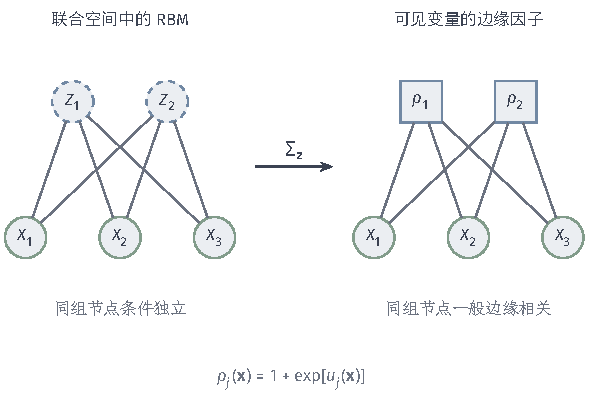
\includegraphics[width=99.653mm]{figures/09-probabilistic-graphical-models/04-models/tikz/pgm-energy-models-rbm/figure.pdf}
  \caption{RBM的条件分解与隐藏消元。左侧仅有跨组边，固定一组时另一组条件独立；右侧把两个隐藏节点消去，两个因子$1+\exp[u_j(\bm{x})]$各涉及三个可见变量。一元可见偏置势在两侧均省略。可见边缘仍可能相关。}
  \label{fig:pgm-energy-models-rbm}
\end{figure}

取两个可见节点和一个隐藏节点，偏置均为零，$W_{1,1}=W_{2,1}=\log2$。可见权重为$e^{-F(\bm{x})}=1+2^{x_1+x_2}$，配置$(0,0),(0,1),(1,0),(1,1)$的权重依次为$2,3,3,5$，总和为$13$。给定$(x_1,x_2)=(1,1)$，隐藏状态为$1$的概率是$4/5$。给定$z=0$时，两可见节点独立、取$1$概率各为$1/2$；给定$z=1$时，该概率各为$2/3$。消去隐藏状态后，$p(X_1=X_2=1)=5/13$与$p(X_1=1)p(X_2=1)=(8/13)^2$相差$1/169$，独立性没有保留。

单个可见配置的自由能求值为$O(d_{\mathrm{v}}m)$，其权重总和$Z_{\bm{\theta}}=\sum_{\bm{x}}e^{-F_{\bm{\theta}}(\bm{x})}$通常仍需指数计算。枚举较小的一组、解析消去另一组虽可减少运算，仍含$2^{\min(d_{\mathrm{v}},m)}$规模。RBM使完整可见配置下的隐藏后验可算，没有普遍消除联合归一化成本。部分可见量未测时，$p(\bm{z}\mid\bm{x}_{\mathrm{obs}})$也未必保有上述独立Bernoulli分解。

这两个块条件可以构成\term{交替Gibbs采样}（alternating Gibbs sampling）：固定一组，独立随机抽取另一组，再交换两组。算法~\ref{alg:pgm-energy-models-rbm-gibbs}传递的是抽到的二值状态；若直接传递概率，所得确定性迭代已不再使用这个Gibbs核。

\begin{algorithm}[RBM的一段交替Gibbs链]
  \label{alg:pgm-energy-models-rbm-gibbs}
  \begin{algorithmic}[1]
    \Require 固定的有限参数$\bm{\theta}$，初始状态$\bm{x}^{(0)}$，步数$k\geq1$
    \Ensure 链状态$\bm{x}^{(1)},\ldots,\bm{x}^{(k)}$
    \For{$t=0,\ldots,k-1$}
      \State 固定$\bm{x}^{(t)}$，按式~\eqref{eq:pgm-energy-models-rbm-conditionals}独立抽取各$Z_j^{(t+1)}$
      \State 固定$\bm{z}^{(t+1)}$，独立抽取各$X_i^{(t+1)}$
    \EndFor
  \end{algorithmic}
\end{algorithm}

固定有限参数下，每个块条件概率都在$0$与$1$之间，可见状态链因而能到达任意配置，并有自转移。交替Gibbs核保持$p_{\bm{\theta}}(\bm{x})$不变，有限不可约、非周期链的分布遂长期收敛到它；这并未给出小$k$充分混合的保证（参见第~\ref{chap:pgm-sampling}章）。完整一次更新为$O(d_{\mathrm{v}}m)$，强权重形成的近确定条件可能使链长期停留在同一模式。

RBM仍以可见数据的似然为学习目标。利用式~\eqref{eq:pgm-energy-models-free-energy}，其负对数似然可以直接写为
\begin{equation}
  \mathcal{L}_{\mathrm{RBM}}(\bm{\theta})
    =\sum_{r=1}^n F_{\bm{\theta}}(\bm{x}_r)
       +n\log Z_{\bm{\theta}}.
  \label{eq:pgm-energy-models-rbm-nll}
\end{equation}
自由能可算只完成了数据项，配分函数项仍比较所有可见配置。训练一个权重时，需要提高数据配置的概率，同时扣除模型自身的联合统计。对单条数据$\bm{x}$，潜变量似然梯度在RBM中写为（通用推导参见第~\ref{chap:pgm-parameter-learning}章）
\begin{equation}
  \frac{\partial\log p_{\bm{\theta}}(\bm{x})}
       {\partial W_{i,j}}
    =x_i\,p_{\bm{\theta}}(Z_j=1\mid\bm{x})
      -\mathbb{E}_{p_{\bm{\theta}}}[X_iZ_j].
  \label{eq:pgm-energy-models-rbm-gradient}
\end{equation}
数据项由隐藏条件概率精确取得，模型项则通常需要采样。多条记录对数据项求平均，偏置的梯度对应一阶统计量。RBM简化的是给定数据的后验计算，模型期望仍然存在。重构误差与似然也有不同含义：慢混合的短链容易留在起始数据附近，却可能没有正确分配不同模式的概率质量\scite{pgm-energy-models-hinton2010}

为落实权重更新，记当前链给出的模型联合统计估计为$\widehat{m}_{i,j}\approx\mathbb{E}[X_iZ_j]$，则沿平均对数似然梯度方向的近似更新写为
\[
  W_{i,j}\leftarrow W_{i,j}+\eta\left[
      \frac1n\sum_{r=1}^n
            x_{r,i}\,p_{\bm{\theta}}(Z_j=1\mid\bm{x}_r)
       -\widehat{m}_{i,j}\right].
\]
可见偏置用经验$x_i$减模型$\mathbb{E}[X_i]$，隐藏偏置用数据后验概率均值减模型$\mathbb{E}[Z_j]$。梯度统计允许对已经条件化的隐藏状态取精确期望；这不改变前述采样算法需要传递随机状态的要求。参数更新后，链的目标分布也随之改变，下一轮需按新参数继续采样。

对比散度从数据配置启动短链，用终点统计替代模型期望；持久对比散度沿用上轮链状态，以跟踪缓慢变化的模型。二者近似了取得模型期望的过程，有限步更新未必等于精确似然梯度。短链终点分布随参数变化，忽略其分布导数也是这种更新不能一般性地解释为某个固定目标精确梯度的原因之一；持久链能否跟上模型变化，还取决于混合速度与参数更新尺度（参见第~\ref{chap:pgm-parameter-learning}章）。因此，训练流程应按固定参数采样、估计模型统计、计算数据减模型梯度、更新参数的顺序理解，短链重构好不能替代似然或混合检查。

图~\ref{fig:rbm-alternating-sampling-and-gradient}按这一顺序区分概率、抽样状态与训练统计：先固定参数运行交替链、估计模型统计，再用数据统计减模型统计更新参数。

\begin{figure*}[htbp]
  \centering
  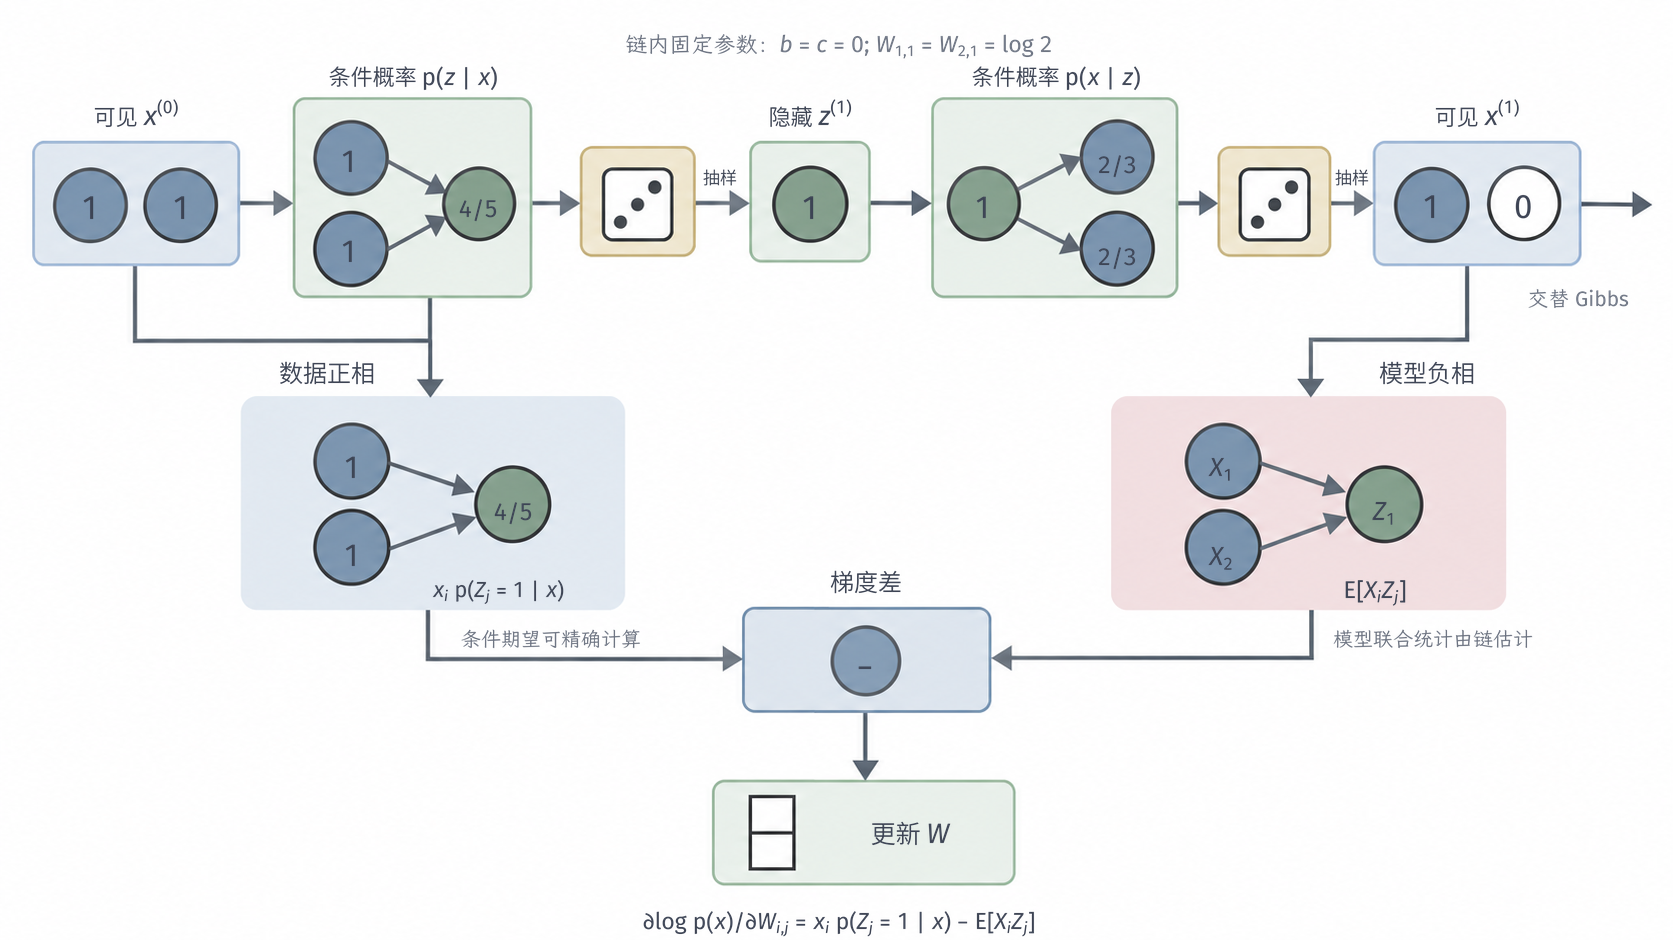
\includegraphics[width=141.647mm]{figures/09-probabilistic-graphical-models/04-models/generated/rbm-alternating-sampling-and-gradient/figure.png}
  \caption{二值RBM中的抽样状态和训练统计。取$b=c=0$、$W_{1,1}=W_{2,1}=\log2$，可见状态$(1,1)$对应隐藏条件概率$4/5$；若抽到$z=1$，可见单元的条件概率各为$2/3$，下一状态可以是$(1,0)$。图中概率与抽样值分别标出。似然梯度以可算的数据统计减去采样估计的模型联合统计，单步重构不能证明混合已完成。}
  \label{fig:rbm-alternating-sampling-and-gradient}
\end{figure*}

\section{给定输入的结构化输出预测}
\label{sec:pgm-energy-models-conditional-models}

若温度、历史摘要和传感器类型已经给定，检测任务可以只预测异常标签。为这些输入另拟联合分布未必是必要步骤。条件能量将输入作为已知量，专门表达标签之间的相容性；标签配置共同竞争概率质量，仍须处理全局输出归一化。

\subsection{标签相容关系与条件随机场}
\label{sec:pgm-energy-models-crf-definition}

前面联合模型要对输入和标签的所有配置一起归一化；但在“输入已知、只预测标签”的任务里，为复杂的输入分布建模既费力又与预测目标无关。我们真正想表达的是：在给定输入的前提下，一组标签如何\emph{彼此相容}（相邻词的词性倾向一致、相连位置的标签倾向连续）。于是把输入当作固定条件，只用一个无向图刻画标签之间的条件依赖、并仅在标签空间归一化即可。固定输入之后，可以用无向图规定标签的条件独立关系。满足这种Markov性质的条件分布称为\term{条件随机场}（conditional random field, CRF），通常通过输入相关的团势构造：
\begin{equation}
  \begin{aligned}
    p_{\bm{\theta}}(\bm{y}\mid\bm{x})
      &=\frac{1}{Z_{\bm{\theta}}(\bm{x})}
          \prod_{C\in\mathcal{C}}
             \psi_{\bm{\theta},C}(\bm{y}_C,\bm{x}),\\
    E_{\bm{\theta}}(\bm{y},\bm{x})
      &=-\sum_{C\in\mathcal{C}}
             \log\psi_{\bm{\theta},C}(\bm{y}_C,\bm{x}).
  \end{aligned}
  \label{eq:pgm-energy-models-crf-factors}
\end{equation}
该图只以输出变量为节点。固定输入，若$S$分离$A$、$B$，则$\bm{Y}_A\perp\bm{Y}_B\mid(\bm{Y}_S,\bm{x})$。完整输入可以被多个势或序列编码器读取；标签作用域由一个势同时涉及哪些未知标签决定，不能从输入编码器的连线推定。

既有联合Markov模型$p(\bm{x},\bm{y})$条件化后也能给出CRF形式，直接条件拟合则只学习$p(\bm{y}\mid\bm{x})$，不同时约束$p(\bm{x})$。反向组成联合分布时，必须为CRF另选输入分布。输入缺失需要边缘化时，同样缺少其分布，单凭条件标签模型无法完成这项查询。

常用的线性形式为$\log\psi_{\bm{\theta},C}=\bm{\theta}^\top\bm{f}_C(\bm{x},\bm{y}_C)$，各作用域可以共享参数。给定完整标签记录$\{(\bm{x}_r,\bm{y}_r)\}_{r=1}^n$，比较观测特征得分与该输入下全部标签的权重总量，条件对数似然为
\begin{equation}
  \ell_{\mathrm{cond}}(\bm{\theta})
    =\sum_{r=1}^n
       \left[
        \sum_C\bm{\theta}^\top
                    \bm{f}_C(\bm{x}_r,\bm{y}_{r,C})
        -\log Z_{\bm{\theta}}(\bm{x}_r)
       \right].
  \label{eq:pgm-energy-models-crf-likelihood}
\end{equation}
把整条记录的特征和记为$\bm{f}(\bm{x},\bm{y})=\sum_C\bm{f}_C(\bm{x},\bm{y}_C)$，条件似然梯度为
\begin{equation}
  \nabla_{\bm{\theta}}\ell_{\mathrm{cond}}
    =\sum_{r=1}^n\left[
        \bm{f}(\bm{x}_r,\bm{y}_r)
        -\mathbb{E}_{p_{\bm{\theta}}(\bm{Y}\mid\bm{x}_r)}
                 [\bm{f}(\bm{x}_r,\bm{Y})]\right].
  \label{eq:pgm-energy-models-crf-gradient}
\end{equation}
不同输入一般给出不同配分函数。学习时先固定参数，针对每个输入计算标签边缘及期望特征，再累加观测特征与模型期望之差，最后更新参数。因此，训练中重复执行的是标签图的推断，输入本身不参与这一步的归一化。

若采用二次正则化，可以最小化$-\ell_{\mathrm{cond}}(\bm{\theta})+\frac\lambda2\lVert\bm{\theta}\rVert_2^2$，其梯度为$-\nabla\ell_{\mathrm{cond}}+\lambda\bm{\theta}$。一次梯度下降由这两个可区分的部分组成：条件统计差负责拟合标签，正则项控制参数大小。训练后，预测整组最相容标签求的是$\arg\max_{\bm{y}}p_{\bm{\theta}}(\bm{y}\mid\bm{x})$，若要报告单个标签的不确定性，则须计算相应边缘概率，不能用最优配置分量替代。

固定特征、完整标签的线性参数化使对数似然为凹函数，未正则化目标能否取得有限最优解仍取决于可分离性等条件。对有限输出空间和有限特征值，取$\lambda>0$并惩罚全部参数可使上述负对数似然目标严格凸且在参数范数趋于无穷时增长；可训练神经特征或未观测标签的边缘化则不保留一般凹性结论（梯度推导参见第~\ref{sec:pgm-parameter-learning-conditional}节）。以时间或序列位置重复输出关系时，可以进一步得到链与片段模型，其详细计算见第~\ref{chap:pgm-dynamic-undirected}章。CRF的完整表述见Sutton与McCallum\scite{pgm-energy-models-sutton2012}

二维位置或相互连接的设备可能需要保留链之外的标签关系，标签图因而可能成环。团树可以精确汇总它的概率（参见第~\ref{chap:pgm-junction-tree}章），成本取决于消元后的作用域。标签数为$K$、所用消元序诱导宽度为$w$时，主要计算一般含$K^{w+1}$规模。简单环宽度仍小，不必一律近似；密集关系或大型高阶作用域则可能超出可用资源。

宽图难以精确处理时，可近似边缘或最优配置。平均场、环置信传播及采样用于概率与期望，最大化松弛、图割或整数优化针对最优配置（参见第~\ref{chap:pgm-variational}、\ref{chap:pgm-sampling}章）。后一个问题的解不会自动给出前一个问题的概率。环消息可能不收敛，收敛值也未必是精确边缘；据此训练时，须说明使用了近似梯度或配分函数。

\subsection{关系实例上的共享预测}
\label{sec:pgm-energy-models-general-relational}

和联合模型里的MLN类似，条件模型也常遇到“同一套标签相容规则要作用到一张大图里的许多实体上”的情况，例如社交网络里每对好友之间都复用同一条“标签倾向一致”的势。这时可以把CRF的标签势也写成跨实体共享参数的模板，用同一组参数处理数量不定的实例。当同类设备关系需要反复用于许多实体时，关系CRF可以把式~\eqref{eq:pgm-energy-models-crf-factors}中的输出作用域写成共享模板。设备属性、已知连接及图结构属于输入，待预测标签才是未知变量。

例如，每个设备有标签$Y_i$，属性形成一元势，每条已知连接复用同一相邻标签势。若输入$\bm{x}$进一步确定模板$r$的实例集$\mathcal{I}_r(\bm{x})$，各实例的得分相加为
\begin{equation}
  E_{\bm{\theta}}(\bm{y},\bm{x})
   =-\sum_r\sum_{g\in\mathcal{I}_r(\bm{x})}
        \bm{\theta}_r^\top
             \bm{f}_r(\bm{x}_g,\bm{y}_g).
  \label{eq:pgm-energy-models-relational-crf}
\end{equation}
实例$g$选定具体实体及关系作用域，$\bm{x}_g$收集已知特征，$\bm{y}_g$包含参与的未知标签。共享参数$\bm{\theta}_r$接收各实例的学习统计；实例可能重叠，不能因此当作独立记录。Taskar等人的关系Markov网络给出了这种条件分布与集体分类的代表构造\scite{pgm-energy-models-taskar2002}

关系共享也需要明确整条训练记录的边界。令第$s$条记录$\bm{x}_s$给出一张关系图及其已知属性，$\bm{y}_s$给出该图的完整标签；不同记录按独立图样本处理，一张图内部的标签仍可相关。把模板$r$的实例特征和记为
\[
  \bm{F}_r(\bm{x},\bm{y})
    =\sum_{g\in\mathcal{I}_r(\bm{x})}
                  \bm{f}_r(\bm{x}_g,\bm{y}_g).
\]
本地条件目标及共享参数的梯度为
\begin{equation}
  \begin{aligned}
    \ell_{\mathrm{rel}}(\bm{\theta})
      &=\sum_{s=1}^n\left[
           \sum_r\bm{\theta}_r^\top\bm{F}_r(\bm{x}_s,\bm{y}_s)
           -\log Z_{\bm{\theta}}(\bm{x}_s)\right],\\
    \nabla_{\bm{\theta}_r}\ell_{\mathrm{rel}}
      &=\sum_{s=1}^n\left[
          \bm{F}_r(\bm{x}_s,\bm{y}_s)
          -\mathbb{E}_{p_{\bm{\theta}}(\bm{Y}\mid\bm{x}_s)}
                        [\bm{F}_r(\bm{x}_s,\bm{Y})]\right].
  \end{aligned}
  \label{eq:pgm-energy-models-relational-learning}
\end{equation}
每轮先在各输入图上推断标签边缘，再汇总同模板全部实例的统计差，沿梯度更新$\bm{\theta}_r$；需要正则化时加入前节相应项。只有一张关系图时也可以写出$n=1$的条件目标，但不能把它的重叠实例数量直接当作独立样本量。预测新图时，先按该图的已知关系建立实例，再求联合最优标签或标签边缘。

MLN与关系CRF都能共享落地模板，区别在于哪些命题参与归一化。前者为选定域上的命题配置建立联合分布，连接可以成为未知变量；后者在这里固定属性和连接，只归一化待预测标签。对MLN的已知命题条件化可以得到相应的条件能量，但一般关系CRF并未同时给出这些输入命题的联合分布。这个区别来自概率任务，不能只从二者都使用模板推断它们等价。

关系势错误也会沿集体推断传播。若所有连接都奖励同标签，而实际常连接不同故障类型，多个节点可能共同偏移；高连接度还使一个位置重复参与许多势。需要检查特征与共享方式，延长消息迭代无法修复这种错设。连接仅作为已知输入时，其生成分布仍未定义，标签推断不能自行扩展为未知连接生成。

评价须说明预测发生在同一张关系图还是新图。同图中已标注、未标注节点的划分属于传导任务，与预测全新独立图不同；测试标签不得借邻域特征进入训练。部分训练标签未观测时，条件似然分子也要边缘化它们，训练增加后验推断并通常失去凹性。共享关系模式可以合并信息，相关性、划分泄漏及推断误差仍要分别控制。

\section{联合与条件模型的关系及计算选择}
\label{sec:pgm-energy-models-comparison}

本章介绍的模型看似各成一家——Ising、GMRF、玻尔兹曼机、RBM、神经能量、MLN、CRF，但它们其实是在同一套“能量＋配分函数”框架上，通过少数几种操作变换得到的：换一种状态编码、删去一些边、引入并边缘化隐藏变量、换掉势的函数形式，或把归一化范围从全部变量改成只对标签。看清这些操作分别保留了什么、改变了什么，就能把这些模型放到一张关系图里，而不必孤立记忆。前面的模型可以通过具体构造联系起来。表~\ref{tab:pgm-energy-models-relations}把重新编码、限制结构、隐藏边缘化、改变参数化和条件化分别列出；每一种操作保留的概率对象不同，因而不能统一理解为简单的模型包含关系。

\begin{table*}[htbp]
  \centering
  \small
  \begin{tabularx}{\linewidth}{p{28mm}p{46mm}X}
    \toprule
    起点与结果 & 具体操作及条件 & 保留与改变的内容\\
    \midrule
    二类Potts与Ising & 类别重编码为$\{-1,+1\}$，耦合与一元偏好换算 & 联合分布不变，能量可相差常数；多类Potts不直接沿用此二值换算\\
    二值成对模型与BM & 改用$0/1$编码，并指定哪些节点隐藏 & 全部节点上的成对联合形式保留；只观察部分节点时增加隐藏后验与边缘化\\
    BM到RBM & 令可见组内、隐藏组内耦合均为零 & 得到二部子模型，块条件与自由能可算，联合归一化仍可能困难\\
    RBM到可见高阶势 & 对隐藏节点求和 & 保留可见边缘分布，成对联合分解可变成高阶可见势\\
    局部势到神经势 & 在原作用域内替换势的函数族 & 原图的分解与相应条件独立性保留；扩大网络输入作用域则须重新检查图结构\\
    重复逻辑势到MLN模板 & 用逻辑真值计数指定落地势及共享权重 & 共享描述压缩参数和规则写法，落地后仍是联合能量模型\\
    联合模型到CRF形式 & 固定输入，只在输出上重新归一化 & 得到该联合模型的条件分布；单独的CRF不决定输入分布\\
    \bottomrule
  \end{tabularx}
  \caption{本章模型之间的构造关系。等价编码、子模型限制、边缘化和条件化是不同操作，所保留的分布与计算便利须分别核对。}
  \label{tab:pgm-energy-models-relations}
\end{table*}

跨章比较同样要指定对象。第~\ref{chap:pgm-static-directed}章的因子分析与概率PCA通过隐藏因子构造低秩加对角的协方差，GMRF则通过精度零元素表达条件独立性；固定低潜维数与稀疏图时，两种受限模型族一般不互相包含，允许完整图时则都属于非退化高斯分布。有向潜变量模型在局部条件可采样时，可以沿祖先顺序生成联合样本，给定观测后的隐藏后验却可能复杂；RBM在完整可见数据下有解析隐藏后验，但生成仍需处理无向联合分布的采样问题。两者各自简化了不同方向的计算。

模型的区别还可以按归一化变量、可见信息及可利用运算逐项比较。表~\ref{tab:pgm-energy-models-comparison}汇总代表设定，所列属性允许组合；例如采用神经高阶势的关系CRF，仍按给定输入的标签空间归一化。这些名称不是互斥类别。

\begin{table*}[htbp]
  \centering
  \small
  \begin{tabularx}{\linewidth}{p{27mm}p{19mm}p{24mm}p{24mm}X}
    \toprule
    代表设定 & 归一化对象 & 变量与潜变量 & 势的作用域 & 可计算性与主要限制\\
    \midrule
    Ising／Potts & 全部状态 & 离散；此处全观测 & 一元、成对 & 树上精确；一般图的全局求和与强耦合采样可能昂贵\\
    高斯MRF & 全部状态 & 连续；此处全观测 & 二次能量 & 正定精度下可解析归一化；矩阵填充与单峰限制\\
    BM／RBM & 可见与隐藏状态 & 二值；含潜变量 & 联合空间成对 & RBM的块条件与自由能可算，联合配分函数一般仍难\\
    神经联合能量 & 全部状态 & 可离散或连续；潜变量可选 & 局部或全局 & 网络求值不等于归一化；尾部、采样和学习偏差均需控制\\
    MLN & 落地命题配置 & Boolean；可有未观测命题 & 模板决定阶数 & 参数共享不消除落地数量及推断宽度的增长\\
    一般图关系CRF & 给定关系输入的标签 & 此处离散；标签可缺失 & 成对或高阶 & 低宽度可精确；宽图依赖近似推断且须重复用于学习\\
    \bottomrule
  \end{tabularx}
  \caption{本章代表模型的归一化与计算条件。潜变量、势阶数和参数化允许组合，条件模型也可定义连续输出；表中只列本章展开的设定。}
  \label{tab:pgm-energy-models-comparison}
\end{table*}

先按查询选择联合或条件对象。若查询涉及输入的生成或概率补全，还需为输入提供概率模型；始终给定输入而只预测标签时，可以直接学习条件分布。输出依然全局归一化，复杂标签图可能仍难以求和，且不同训练输入各有$Z_{\bm{\theta}}(\bm{x})$。

表达能力要同时看势的函数形式和未知变量作用域。GMRF能借二次结构处理环，却仅表示单峰高斯；RBM的成对联合势可诱导高阶边缘，归一化仍可能昂贵。计数高阶势能用卷积，任意高阶表却需指数存储。局部神经势丰富函数形状并保留原图，全局网络则可能失去稀疏分解，不能只按“成对”或“神经”判断可表达范围与代价。

收敛性分析要区分优化目标与计算该目标的误差。完整离散模型需要模型期望，BM还需数据隐藏后验，RBM只简化后者；神经能量通常依靠负样本或输入导数。线性固定特征CRF有凹似然，但期望是否能精确计算还取决于输出图，训练又需要反复执行这种推断。神经参数或隐藏标签不保留一般凹性。应检查有限最优解、优化停止与近似误差，短链重构或单个训练损失不足以说明收敛。

泛化性需要在未参与拟合和调参的数据上评价，并固定预测单位。条件模型可比较同一留出集上按记录平均的负对数似然，值越小越好；单点标签错误与整组标签错误评价不同输出单位，不能互换。关系模型还要区分同图传导与新图预测。联合模型若用留出似然评价，须取得可比较的配分函数估计并报告其误差；训练目标下降本身不保证这些预测指标改善。

\section{本章小结}
\label{sec:pgm-energy-models-summary}

本章围绕“用无向的相容性给整组状态建模”展开，最核心的认识是：局部势本身不是概率，只有经过全局共同归一化才能形成整组状态的概率，而归一化范围决定了模型是联合的还是条件的。局部相容权重经过共同归一化，才能形成整组状态的概率；能量是权重的负对数写法，添加常数不改分布。三位置联合例子的权重总和为$32$，展示了局部耦合怎样改变整组状态的概率。固定输入后也可以改变标签势，再对输出单独归一化；输入本身无需生成分布。

联合与条件划分归一化对象，其他属性可在其内部组合。潜变量使简单联合作用产生复杂边缘，RBM的二部限制使隐藏后验与自由能可算，联合配分函数仍是训练难点。高阶势及关系模板表达整体约束，也增加作用域、落地规模和可行性要求；神经能量需另查积分尾部及近似学习误差。

固定输入并不意味着标签独立。一般标签图的查询受消元宽度限制；若局部关系沿序列重复，则可利用时间接口组织消息，详见第~\ref{chap:pgm-dynamic-undirected}章。回答开篇问题时，先决定是否需要输入的生成分布，再按所需相互作用选择局部结构，最后确认归一化、推断与学习的成本。表达能力、求解保证和未见数据的预测评价要分别核对。

序列也可以采用有向生成模型：先规定潜状态演化，再为测量定义发射分布，链上的求和与最大化仍可复用（参见第~\ref{chap:pgm-dynamic}章）。这样的观测模型为未来测量的概率预测提供依据；本章固定输入的标签CRF则只规定标签条件分布，未给输入读数建立生成机制。

第~\ref{chap:pgm-generative}章进一步比较潜变量生成、可逆变换和逐步去噪。连接这些模型时，仍应分别询问生成过程是否易于执行、归一化密度是否可算，以及给定观测后的后验是否需要近似。本章的能量形式提供了表达相容性的方法，但并未同时保证这三项计算都容易。

\paragraph{扩展阅读}
Bishop的PRML和Murphy的教材可继续用于学习能量分布及采样训练。建议分别追踪三个计算对象：配置得分、归一化概率、梯度中的模型期望，并核对何种结构使每项可算；得分容易求值不代表概率和期望也容易求值\scite{bishop2006,pgm-murphy2012}
